\documentclass{egpubl}

% --- for  Annual CONFERENCE
% \ConferenceSubmission % uncomment for Conference submission
% \ConferencePaper      % uncomment for (final) Conference Paper
% \STAR                 % uncomment for STAR contribution
% \Tutorial             % uncomment for Tutorial contribution
% \ShortPresentation    % uncomment for (final) Short Conference Presentation
%
% --- for  CGF Journal
 \JournalSubmission    % uncomment for submission to Computer Graphics Forum
% \JournalPaper         % uncomment for final version of Journal Paper
%
% --- for  CGF Journal: special issue
% \SpecialIssueSubmission    % uncomment for submission to Computer Graphics Forum, special issue
% \SpecialIssuePaper         % uncomment for final version of Journal Paper, special issue
%
% --- for  EG Workshop Proceedings
% \WsSubmission    % uncomment for submission to EG Workshop
 %\WsPaper         % uncomment for final version of EG Workshop contribution
%
 \electronicVersion % can be used both for the printed and electronic version

% !! *please* don't change anything above
% !! unless you REALLY know what you are doing
% ------------------------------------------------------------------------

% for including postscript figures
% mind: package option 'draft' will replace PS figure by a filname within a frame
\ifpdf \usepackage[pdftex]{graphicx} \pdfcompresslevel=9
\else \usepackage[dvips]{graphicx} \fi

\PrintedOrElectronic

% prepare for electronic version of your document
\usepackage{t1enc,dfadobe}
%\usepackage{url}
\usepackage{algorithm2e}
\usepackage{mathptmx}
\usepackage{graphicx}
\usepackage{times}
\usepackage[usenames,dvipsnames,svgnames]{xcolor}
\usepackage{subfigure}
\usepackage{flushend}
\usepackage[compact]{titlesec}
\usepackage[normalem]{ulem}

\usepackage{egweblnk}
\usepackage{cite}


\def\etal{\textit{et al.}}
\definecolor{MyGreen}{rgb}{0,0.7,0}
\definecolor{MyWhite}{rgb}{1,1,1}
\definecolor{MyGray}{rgb}{0.5,0.5,0.5}
\definecolor{LightGray}{rgb}{0.7,0.7,0.7}
\definecolor{DarkGray}{rgb}{0.3,0.3,0.3}
\definecolor{DarkYellow}{rgb}{0.7,0.7,0.0}
\definecolor{MyNavyBlue}{rgb}{0.2,0.3,0.7}
\definecolor{darkgreen}{rgb}{0,0.55,0}
\newcommand{\black}[1]{{\color{Black} #1}}
\newcommand{\white}[1]{{\color{MyWhite} #1}}
\newcommand{\gray}[1]{{\color{MyGray} #1}}
\newcommand{\red}[1]{{\color{red} #1}}
\newcommand{\green}[1]{{\color{MyGreen} #1}}
\newcommand{\blue}[1]{{\color{MyNavyBlue} #1}}
\newcommand{\yellow}[1]{{\color{DarkYellow} #1}}
\newcommand{\maybe}[1]{\yellow{#1}}
\newcommand{\rout}[1]{\red{\sout{#1}}}
\newcommand{\repl}[2]{\rout{#1} \green{#2}}
\newcommand{\fix}[1]{\red{\emph{(#1)}}}
\newcommand{\Fix}[1]{\begin{itemize} \renewcommand\labelitemi{\red{--}} \item \red{#1} 
\end{itemize}}


\newcommand{\todo}[1] {\textbf{[~}\textcolor {red}{#1}\marginpar{\textcolor {red}{\centerline{{\Huge \textbf{!}}}}}\textbf{~]}}
\newcommand{\question}[1] {\textbf{[~}\textcolor {darkgreen}{#1}\marginpar{\textcolor {darkgreen}{\centerline{{\Huge \textbf{!}}}}}\textbf{~]}}
\newcommand{\diff}[1]{\textcolor{blue}{#1}}

\setlength\fboxsep{0pt}

% end of prologue

\title[Urban Search \& Rescue Mission Planning Support]{A Visualization-Based Analysis System\\for Urban Search \& Rescue Mission Planning Support}

\author[Bock \etal]{
    Alexander Bock$^1$, \AA sa Svensson$^2$, Alexander Kleiner$^3$, Jonas Lundberg$^2$, and Timo Ropinski$^{1,4}$\\%
    $^1$ Scientific Visualization Group, Link\"oping University \\%
    $^2$ Graphic Design Group, Link\"oping University \\%
    $^3$ iRobot, Pasadena, CA\\%
    $^4$ Visual Computing Group, Ulm University
}   

%% Uncomment below to disable the manuscript note
%\renewcommand{\manuscriptnotetxt}{}

%% Copyright space is enabled by default as required by guidelines.
%% It is disabled by the 'review' option or via the following command:
% \nocopyrightspace

%%%%%%%%%%%%%%%%%%%%%%%%%%%%%%%%%%%%%%%%%%%%%%%%%%%%%%%%%%%%%%%%%%%%%%%%%%%%%%%%%%%%%%%%%%%
%%%%%%%%%%%%%%%%%%%%%%%%%%%%%%%%%%%%%%%%%%%%%%%%%%%%%%%%%%%%%%%%%%%%%%%%%%%%%%%%%%%%%%%%%%%

\begin{document}

\teaser{
%  \newcommand{\abTeaserImageWidth}{0.31\linewidth}
%  \newcommand{\abTeaserImageHeight}{0.245\linewidth}
  \newcommand{\abTeaserImageWidth}{0.31\linewidth}
  \newcommand{\abTeaserImageHeight}{\abTeaserImageWidth}
	\centering
	\subfigure[Voxelized point cloud rendering enabling an improved awareness of an office building.]{
		\fbox{\includegraphics[width=\abTeaserImageWidth, height=\abTeaserImageHeight]{figures/image1.jpg}}\label{fig:teaser:1}
	}
	\hfill
	\subfigure[Viable paths through buildings of Tohoku University with two hazardous areas.]{
		\fbox{\includegraphics[width=\abTeaserImageWidth, height=\abTeaserImageHeight]{figures/image2.jpg}}\label{fig:teaser:2}
		\label{fig:teaser:2}
	}
	%\hfill
	%\subfigure[Top-down view of the area providing contextual information.]{
	%	\fbox{\includegraphics[height=0.2375\linewidth]{figures/image2-overview.jpg}}\label{fig:teaser:3}
	% }
	\hfill
	\subfigure[Path analysis using parallel coordinate plots and profile plots.]{
		\fbox{\includegraphics[width=\abTeaserImageWidth, height=\abTeaserImageHeight]{figures/pcpprofile.png}}\label{fig:teaser:4}
	}
  \caption{Our proposed visualization system applied to a collapsed building at Tohoku University. Different views (a,b) present the incident commander with an understanding of the building, allowing him to select and inspect paths that reach a point of interest. The assessment of the trade-off between paths is supported by a set of interactive visual analysis tools (c).}
  \label{fig:teaser}
}

\maketitle

\begin{abstract}
We propose a visualization system for incident commanders in urban search~\&~rescue scenarios that supports path planning in post-disaster structures. Utilizing point cloud data acquired from unmanned robots, we provide methods for the assessment of automatically generated paths. As data uncertainty and a priori unknown information make fully automated systems impractical, we present the incident commander with a set of viable access paths, based on varying risk factors, in a 3D environment combined with visual analysis tools enabling informed decision-making and trade-offs. Based on these decisions, a responder is guided along the path by the incident commander, who can interactively annotate and reevaluate the acquired point cloud and generated paths to react to the dynamics of the situation. We describe visualization design considerations for our system and decision support systems in general, technical realizations of the visualization components, and discuss the results of two qualitative expert evaluation; one online study with nine search~\&~rescue experts and an eye-tracking study in which four experts used the system on an application case.

\begin{classification}
   \CCScat{I.3.7}{Computer Graphics}{Three-Dimensional Graphics and Realism}{Color, shading, shadowing, and texture}
\end{classification}

\end{abstract}

%\setlength\baselineskip{10.75pt}
\section{Introduction}
Structural damage to inhabited buildings is an ever-present danger. As time-to-rescue is an important factor for victims' survivability, it is important for rescue responders to reach victims in a timely fashion. Planning and executing paths through buildings, however, is difficult as floor plans are usually outdated. Furthermore, unknown structural weaknesses, as well as hazardous environments, may make regions and areas of the building inaccessible. While responders use their knowledge and intuition to spot these hazards while traversing the structure, it is paramount that the \emph{Incident Commander} (IC) can analyze the information and coordinate multiple rescue responders simultaneously. In most protocols regarding \emph{Urban Search~\&~Rescue} (USAR) operations, one IC is responsible for a single building and instructs multiple rescue responders inside. During the mission, the IC creates hand-drawn maps of the building based on descriptions of the rescue responders moving in the building searching for victims. During this step, they might stumble into unknown hazardous areas that threaten the rescuers' lives.

In recent years, technological developments made it possible to use unmanned robots to perform this initial exploration. The robots are equipped with sensors performing detailed scans of the interior, capable of detecting victims, gathering information about hazardous environments, and streaming video to the operator. This data is collated into a map that is presented to the IC to plan access paths to \emph{Points of Interest} (POIs). In most cases, these are potential victim locations, but they can also be other mission critical areas.

In this paper, we propose a system utilizing visualization techniques to increase the IC's awareness of internal structures and support the discovery and analysis of optimal access paths (see Figure~\ref{fig:teaser}). Our system computes an ensemble of access paths from an entry point to the POIs, in which each path is based on varying weighting factors. Data uncertainty and unknown information make it infeasible to employ fully automatic algorithms to detect the globally optimal path as this requires expert knowledge. Instead, our system provides the IC with tools to analyze and compare all available paths in order to make an informed trade-off. We describe system requirements, design considerations, technical realizations, and we discuss how experts perform using the visualizations, how they rate their own understanding, and their preferences for the visualizations.

%Section~\ref{sec:relatedwork} will discuss previous works related to our system with Section~\ref{sec:theory} focussing specifically on the related work with regard to human decision-making. The current workflow alongside our proposed workflow is presented in Section~\ref{sec:workflow}. Section~\ref{sec:overview} provides details about our system.

%%%%%%%%%%%%%%%%%%%%%%%%%%%%%%%%%%%%%%%%%%%%%%%%%%%%%%%%%%%%%%%%%%%%%%%%%%%%%%%%%%%%%%%%%%%
%%%%%%%%%%%%%%%%%%%%%%%%%%%%%%%%%%%%%%%%%%%%%%%%%%%%%%%%%%%%%%%%%%%%%%%%%%%%%%%%%%%%%%%%%%%

\section{Related Work} \label{sec:relatedwork}
\noindent {\bfseries Emergency management.} Much of the visualization-oriented work in the field of emergency management deals with evacuation planning before any disaster has occurred. Notable work was performed by Reddy~\etal, which allows users to analyze possible bottlenecks of escape routes~\cite{EuroVA12:13-17:2012}. Ribarsky~\etal\ presented a system organizing first responders inside intact structures~\cite{Ribarsky:2010}. Kim~\etal\ developed a system enhancing the situational awareness of responders using a mobile visual analytics tool~\cite{Kim:2008}. Many existing planning systems deployed nowadays in USAR scenarios are based on 2D representations~\cite{kleiner_et_al_ssrr09,KohlbrecherMeyerStrykKlingaufFlexibleSlamSystem2011}. Given the 2D map of the environment, one common approach to path planning is to plan the shortest trajectory and to follow this trajectory stepwise. Wirth~\etal\ introduced an exploration strategy and path planner that utilizes occupancy grid maps to reach several targets at the same time~\cite{Wirth2007ETA1}. We generalized their idea to apply a voxelization technique to the point cloud data instead.\\
%
\noindent {\bfseries Indoor navigation.} Fisher and Gellersen provided an extensive survey regarding location technology usable by rescuers for indoor navigation~\cite{fischer2010location}. Pascucci and Setola presented a system designed for hybrid rescue teams consisting of human rescuers and robots~\cite{pascucci2011indoor}. Harris provided an article describing the dangers that rescuers face in a search \& rescue scenario with a focus on indoor tracking~\cite{harris2013way}.\\
%
\noindent {\bfseries Point cloud visualization.} Basic rendering capabilities for point clouds are offered by the widely used Point Cloud Library~\cite{Rusu11ICRA}. There has been work by Richter~\etal\ using a level-of-detail structure to render massive point clouds at high frame rates~\cite{Richter:2010:ORV:1811158.1811178}. Xu~\etal\ showed that non-photorealistic rendering techniques can be applied to point cloud data~\cite{conf/npar/XuC04}. The contour lines in their rendering inspired our rendering algorithm. More recently, Pintus~\etal\ presented a rendering algorithm that enhances features of unstructured point clouds in real-time without preprocessing~\cite{Pintus:2011:RRM:2384495.2384513}. In our system, we use a voxelized representation that raises the level of abstraction and provides an immersive experience for the IC in a similar fashion.

%%%%%%%%%%%%%%%%%%%%%%%%%%%%%%%%%%%%%%%%%%%%%%%%%%%%%%%%%%%%%%%%%%%%%%%%%%%%%%%%%%%%%%%%%%%
%%%%%%%%%%%%%%%%%%%%%%%%%%%%%%%%%%%%%%%%%%%%%%%%%%%%%%%%%%%%%%%%%%%%%%%%%%%%%%%%%%%%%%%%%%%

\section{Decision-Making Theory} \label{sec:theory}
It is crucial to take knowledge about human decision making into account when designing a decision support system. Andrienko and Andrienko showed that, in general, the usage of explorative interactive tools support the decision process~\cite{Andrienko:2003kv}. The theory on \emph{Recognition Primed Decision-making}~(RPD)~by Klein and Calderwood~\cite{KleinCalderwood} states that decision makers tend to evaluate options serially in time-constrained situations; they attempt to find one viable plan rather than attempting to generate and compare numerous plans in parallel. Initially, experts look for similarities to previous situations with a focus on relevant goals, things that were important to monitor, and possible actionable items. Then, they go through a process of mental simulation to consider whether these actions are applicable to the case at hand. They assess the ongoing situation, looking for violations and confirmations of expectations, which may require reframing the situation. Klein and Calderwood suggest that ``displays and interfaces should be centered on decisions rather than around data flows''~\cite{KleinCalderwood}, emphasizing that systems should be built to enhance mental simulations. 

The \emph{Contextual Control Model}~(COCOM) by Hollnagel and Woods~\cite{hollnagel2005joint} describes how people rely on context when making decisions. Humans sometimes act with plans of lower quality, relying on the environment to make decisions opportunistically. The quality of their control can be described as scrambled, opportunistic, tactical, or strategic. The scrambled mode refers to decisions made without any information. In the opportunistic mode, people rely on cues in the local context to decide on their next action. In tactical mode, they have an idea how to achieve their goal before taking action---a plan. In strategic mode, the plan includes coordination with other simultaneous goals. The goal for our system is to raise the quality of control from being opportunistic (as in the current workflow) to being strategic, thus enabling improved decision-making capabilities.

The \emph{Extended Control Model}~(ECOM) describes plans in terms of a tactical level (setting goals), monitoring (making plans and overseeing plans), regulating (managing local resources), and tracking (performing and adjusting actions)~\cite{hollnagel2005joint}. This theory can be used to apprise what kind of planning support a system provides. Moreover, it has been argued by Lundberg~\etal\ that it is important for a system to support resiliency: ``Rather than merely selecting a response from a ready-made table, [the system] must adapt and create a suitable response; either by following ready-made plans for adaptation or by making sense of the situation and create responses during the unfolding event''~\cite{Lundberg2012}. Thus, in addition to supporting foreseeable responses, the system should also be capable of working outside of prepared situations and be able to deal with changing circumstances.

%%%%%%%%%%%%%%%%%%%%%%%%%%%%%%%%%%%%%%%%%%%%%%%%%%%%%%%%%%%%%%%%%%%%%%%%%%%%%%%%%%%%%%%%%%%
%%%%%%%%%%%%%%%%%%%%%%%%%%%%%%%%%%%%%%%%%%%%%%%%%%%%%%%%%%%%%%%%%%%%%%%%%%%%%%%%%%%%%%%%%%%

\section{Incident Commander Workflow} \label{sec:workflow}

\begin{figure}
	\newcommand{\abWorkflowImageHeight}{\columnwidth}
	\centering
	\includegraphics[height=\abWorkflowImageHeight]{figures/workflow.pdf}
	\caption{A schematic timeline overview of the currently employed workflow and our proposed system, showing events (red) and actions (blue) split up into four distinct phases. Utilizing additional actions (yellow) in parallel enables faster exploration and decreased overall time-to-rescue.}
	\label{fig:workflow:workflow}
\end{figure}

In this section, we will first describe the current workflow of the IC and then propose a visualization-enhanced workflow supported by our system (see Figure~\ref{fig:workflow:workflow}). The workflow description is based on the information from the Federal Emergency Management Agency. Roman numerals in the text refer to the corresponding phases in the figure.\\
%
\noindent {\bfseries Current workflow.} The first step for the responders is to explore and secure the area outside the collapsed structure and gather the rescue team (Phase \texttt{I}). No rescuer is allowed to enter the building until this phase is finished, which can take multiple hours (Phase \texttt{II}). Then, the team determines viable entry points, rescuers enter the building and are directed by the IC to perform reconnaissance (Phase \texttt{III}). The rescuers inside the building advance and report their progress to the IC, who draws a two-dimensional map of the interior based on their descriptions (Phase \texttt{IV}). The exploration of these areas expose the rescuer to unknown risks, for example gas leaks or dormant fires. This is a good example of opportunistic control, where decisions are made opportunistically based on feedback from the environment without access to global information. Although responders may recognize situations, decisions regarding the path are limited to the extent of the exploration and their view of the local environment. Global planning is further limited by the limited ability to communicate relevant information, such as turns, accurately to the IC, which causes hand-drawn maps to drift.\\
%
\noindent {\bfseries Visualization-enhanced workflow.} The initial steps of securing the area are the same as in the current workflow. While the responders are securing the building, which is the most time-consuming of the initial tasks, unmanned robots perform the initial reconnaissance of the structure, creating a three-dimensional map of the interior~(yellow actions in Phase \texttt{II}). Furthermore, the robots' sensors are able to detect victims using, for example, thermal cameras and heart beat sensors, but as these measurements are uncertain, false positives and false negatives might occur. The same holds true for hazardous environments like fires, gas leaks, structurally unsafe areas, radiation, or others. Data retrieval and preprocessing are done in parallel while securing the perimeter, so that all information is available when Phase \texttt{III} begins. Based on suggested POIs, the system computes an ensemble of optimal paths through the generated map, thus reducing time-to-rescue (Phase \texttt{IV}) as the rescuers do not need to explore the building to the same extent to find victims, but can advance towards their location immediately. The proposed system applies RPD to the situation and extends the planning from local conditions to higher ECOM levels each rescuer has information about the whole structure.

During path planning, multiple factors must be taken into account. The responder must maintain a safe distance from hazardous environments, avoid overhanging structures that might collapse with a rescuer beneath, and the ground must be stable and level. These variables are extracted from the map and are, thus, uncertain. The IC has to consider trade-offs to choose between alternatives, for example favoring a longer, safer path over a shorter, more dangerous one.

While the IC is instructing the rescuer to follow a specific path, the rescuer feeds back information about victims or new hazards and the IC incorporates this information immediately into the system. This is of high importance as features might not only have been missed by the robots, but might change during the rescue operation. Fires can start or extinguish, additional collapses can make areas inaccessible, or new passages might be created after the initial reconnaissance by removing rubble or breaching walls.

%%%%%%%%%%%%%%%%%%%%%%%%%%%%%%%%%%%%%%%%%%%%%%%%%%%%%%%%%%%%%%%%%%%%%%%%%%%%%%%%%%%%%%%%%%%
%%%%%%%%%%%%%%%%%%%%%%%%%%%%%%%%%%%%%%%%%%%%%%%%%%%%%%%%%%%%%%%%%%%%%%%%%%%%%%%%%%%%%%%%%%%

\section{System Overview} \label{sec:overview}

Combining expertise in visualization, cognitive systems engineering, rescue robotics, and discussions with experts, we determined the following requirements for our system:
\begin{description}
\item[R1] The system must increase spatial awareness by allowing for interactive exploration of the collapsed structure.
\item[R2] The system must enable the IC to interactively annotate the acquired data to react to changing circumstances.
\item[R3] The IC must be able to inspect all suggested access paths, compare them, and make viable trade-offs.
\item[R4] The system must provide the tools for the IC to select his chosen optimal path and support its execution.
\end{description}

To address these requirements, our proposed system, depicted in Figure~\ref{sec:overview:system}, employs multiple linked views. In order to fulfill {\bfseries R1}, our system renders the point cloud interactively while preserving occlusion information and, thus, helping the IC to form a mental model of the building. The IC can seamlessly annotate newly discovered entrances, hazards, POIs, and inaccessible areas directly in the rendering, thus fulfilling {\bfseries R2}. To address {\bfseries R3} and {\bfseries R4}, we integrate a visual representation of the different paths into the 3D visualization, and provide in-depth analysis tools.

The following sections address the individual components of our system. Before the acquired data can be used, the data must be preprocessed (Section~\ref{sec:overview:preprocessing}). Section~\ref{sec:overview:annotation} explains the interactive annotation of the point cloud. We describe the path computation process and the analysis together with comparison metrics in Sections~\ref{sec:overview:pathcomputation} and~\ref{sec:overview:pathanalysis}. Lastly, Section~\ref{sec:overview:3dvisualization} provides details on the considerations that went into designing the visualization components of our system. An earlier version of this system has been previously proposed by the authors~\cite{BKLR14}. The evaluation in that work greatly influenced the subsequent changes.

\begin{figure}
	\newcommand{\abSystemScreenshotWidth}{\columnwidth}
    \centering
    \framebox[\columnwidth][c]{
        \includegraphics[width=\columnwidth]{figures/fig-overview-system2.png}
    }
    \caption{A screenshot of our system in a typical scenario. The center view shows a bird's eye view onto the structure providing contextual information. The right view allows for detailed inspection of different paths and navigation in the three-dimensional environment.}
    \label{sec:overview:system}
\end{figure}


\subsection{Data Preprocessing} \label{sec:overview:preprocessing}
The data retrieved from the unmanned robots is an unstructured point cloud. One issue with rendering point clouds is depth perception and the non-uniform distribution of measured points. To avoid this problem, we perform a binning to obtain a three-dimensional regular voxel data structure. The voxel size is dependent on the scan resolution of the robot, and is a trade-off between resolving smaller details and increasingly noisy data. In our cases, voxel sizes of about 5\,cm were sufficient with regard to this trade-off. We call a measurement in the original point cloud a \emph{point} and refer to a position in the grid-based, binned point cloud as a \emph{voxel}.\\
%
\noindent {\bfseries Attribute derivation.} In the second part, derived attributes are computed on the voxel grid that are later used to determine the set of rescue paths and to support and inform their analysis. Figure~\ref{fig:imageenhancement:colors} shows a selection of these attributes. We compute a \emph{hazard distance field} that denotes the distance to the closest hazard points. The \emph{support field} shows the available supporting area for each voxel. This value determines whether there is enough floor available for a responder to walk on. The \emph{occupancy field} denotes the number of points each voxel is based on. A higher occupancy means that the voxel contains more points in the original point cloud data and thus provides a higher certainty. The \emph{size field} shows for each voxel if a rescuer can fit into the space above the voxel. In the default settings, we calculate two size values, one with the rescuer standing up, and a second while crouching. However, the system is designed to allow easy integration of different geometries, such as additional unmanned robots. In order to compute viable paths, we also need surface orientation information to be able to exclude paths that would be too steep for a rescuer. The steepness of surfaces is approximated by the normal of a least-squares fitted plane based on all the points in the original point cloud that are covered by each voxel.

\subsection{Data Annotation} \label{sec:overview:annotation}
Each voxel can belong to one of five classes and defaults to \emph{Unclassified}. \emph{Start} voxels are accessible entry points. This means that paths can start from any of these points. \emph{POI} voxels are destination points for paths. These indicate locations with a potential victim or another mission-critical element. \emph{Hazard} voxels have been declared as dangerous due to, for example, an ongoing fire or a gas leak. Each hazard area has a normalized severity denoting the danger. Points can be assigned to these three classes either by the initial reconnaissance of the robot or, in a later step, interactively by the IC. \emph{Forbidden} voxels can only be declared by the IC and are areas that are completely out of reach. These points are used when, for example, a corridor collapses after the point cloud acquisition and is not accessible anymore. The classification for each voxel is modified by interacting with the 3D rendering using mouse and keyboard, thus fulfilling {\bfseries R2}. 

\subsection{Path Computation} \label{sec:overview:pathcomputation}
We employ the widely used A* algorithm for the path computations~\cite{4082128}. For the current voxel $x$, the estimated remaining distance to the target is calculated for all unvisited neighboring voxels $y_i$. This value is the accumulated cost to reach $x$, the cost to move from $x$ to $y_i$ given a metric $m$, and the estimated cost to reach the target from $y_i$ using a heuristic. The neighboring voxel with the lowest cost is chosen as the next candidate. When computing a path, the metric $m$ determines the cost of moving from one voxel to its neighbor and, thus, the optimal path. However, it is possible to compute several optimal paths by changing this metric. The metric used in our system is composed of several, weighted sub-metrics and is given by:
%
\begin{equation}
\begin{array}{r@{}l}
m = & \textrm{L}_2(\mathbf{p},\mathbf{q}) + w_h \cdot \textrm{hazard}(\mathbf{q}) + w_s \cdot \textrm{size}(\mathbf{q}) + \vspace*{0.1cm} \\
  & w_n \cdot \textrm{normal}(\mathbf{q},\varphi) + w_{sup} \cdot \textrm{support}(\mathbf{q},n)
\end{array}
\label{eqn:metric}
\end{equation}

\noindent where $w_h$, $w_s$, $w_n$, and $w_{sup}$ are the weights that are varied between different path computations. $\mathbf{p}$ is the current voxel position and $\mathbf{q}$ is the next voxel position under consideration, $\textrm{hazard}(\mathbf{q})$ returns the hazard severity, $\textrm{size}(\mathbf{q})$ is a binary function that determines if there is enough space above voxel $\mathbf{q}$, $\textrm{normal}(\mathbf{q},\varphi)$ computes the surface normal and returns a response between the maximum allowed deviation $\varphi$ and the direction of gravity, and $\mathrm{support}(\mathbf{q},n)$ is the number of supporting voxels, with $n$ being a threshold determining the number of voxels needed to consider $\mathbf{q}$ being supportive.

\begin{figure*}[ht]
	\newcommand{\abSamplingImageWidth}{0.2\textwidth}
	\centering
	\subfigure[After initialization]{
		\includegraphics[width=\abSamplingImageWidth]{figures/adaptive_sampling_1.png}
		\label{fig:sampling:adaptive:1}
	}
	\hfill
	\subfigure[After the first iteration]{
		\includegraphics[width=\abSamplingImageWidth]{figures/adaptive_sampling_2.png}
		\label{fig:sampling:adaptive:2}
	}
	\hfill
		\subfigure[Regions with out subdivision during the next iteration]{
		\includegraphics[width=\abSamplingImageWidth]{figures/adaptive_sampling_3.png}
		\label{fig:sampling:adaptive:3}
	}
	\hfill
		\subfigure[Including the samples generated in (c)]{
		\includegraphics[width=\abSamplingImageWidth]{figures/adaptive_sampling_4.png}
		\label{fig:sampling:adaptive:4}
	}
	\hfill
	\caption{Adaptive sampling in two dimensions. Black dots are recursive samples, white dots are non-recursive, and numbers are identifiers for paths. There is a non-recursive sample for each corner and a recursive sample in the center (a). In each iteration, the central value is checked against each corner value and if they are different, new samples are created (b,c,d).}
	\label{fig:sampling:adaptive}
\end{figure*}


\subsubsection{Adaptive Sampling}
\begin{figure}
	\newcommand{\abSamplingComparisonWidth}{\linewidth}
	\centering
	\subfigure[Regular Sampling] {
		\includegraphics[width=\abSamplingComparisonWidth]{figures/regular_sampling.png}
		\label{fig:sampling:comparison:regular}
	}
	\subfigure[Adaptive Sampling using binary space partitioning] {
		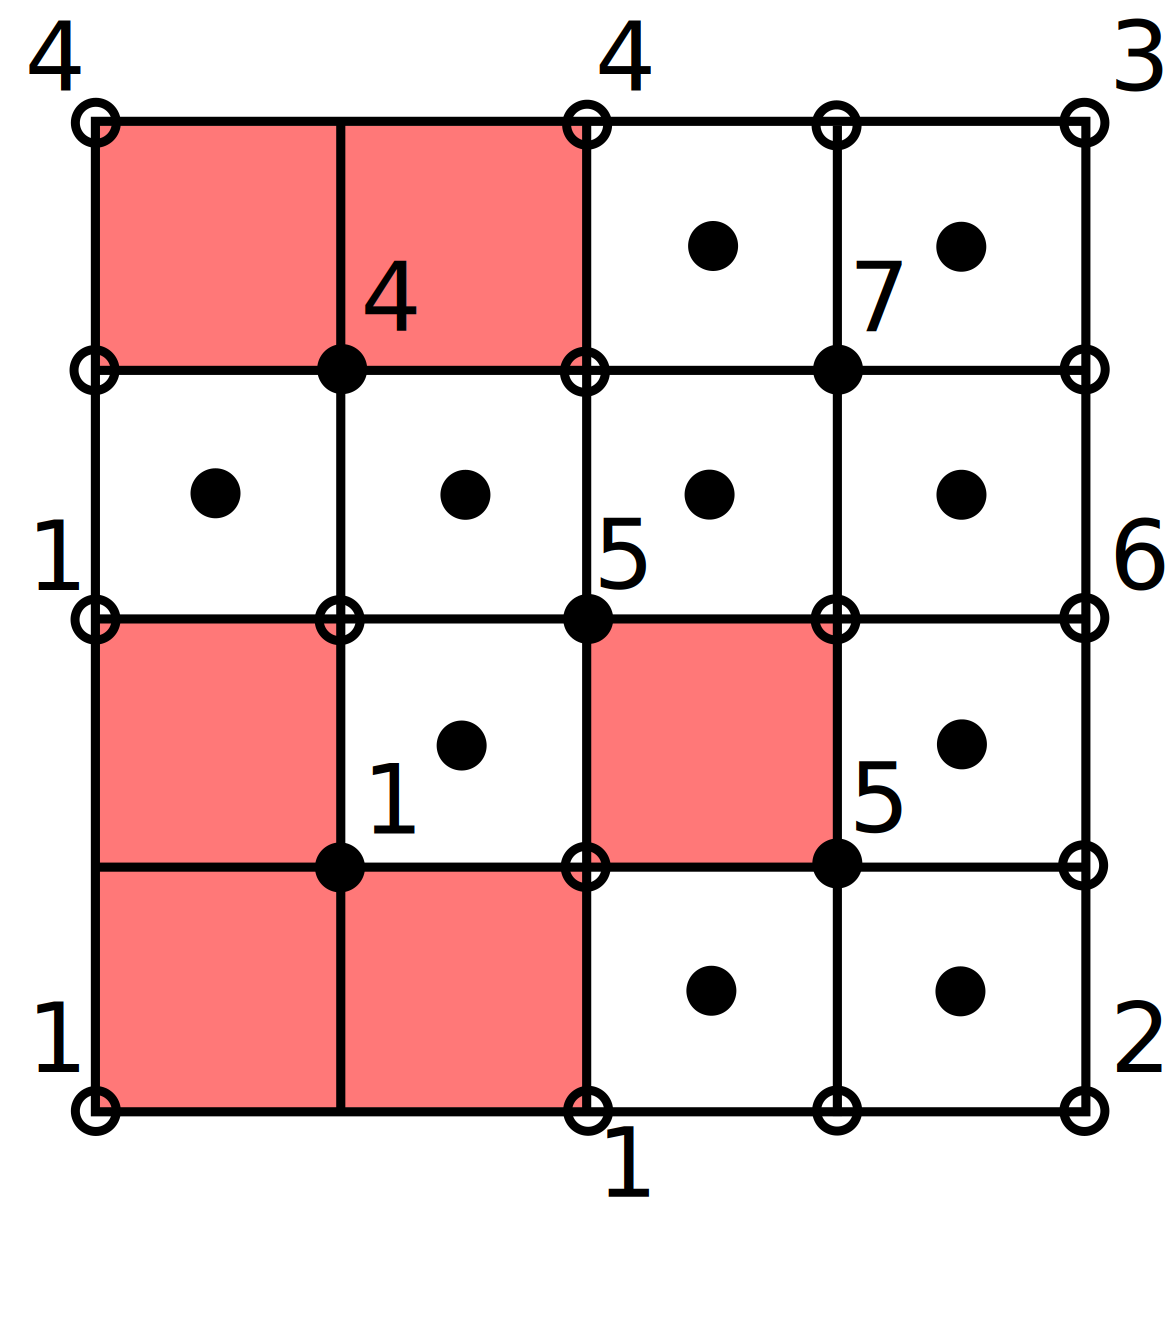
\includegraphics[width=\abSamplingComparisonWidth]{figures/adaptive_sampling.png}
		\label{fig:sampling:comparison:adaptive}
	}
	\caption{Comparison between equidistant and adaptive sampling. Vertical lines correspond to samples, different colors symbolize different paths. With regular sampling, green is oversampled while blue is not sampled at all. The adaptive sampling scheme samples all paths as evenly as possible.}
	\label{fig:sampling:comparsion}
\end{figure}

\begin{algorithm}
Creating $2^d$ non-recursive boundary samples\;
Creating one recursive sample value at 0.5\;
\While{new recursive samples exist}{
	\ForEach{$x$ in non-recursive samples}{
		compute path $p$ using the metric created from $x$\;
		update with path $p$\;
	}
	\ForEach{$x$ in recursive samples}{
		\If{distance $x$ to all corner values $< \epsilon$}{
			break\;
		}
		compute path $p$ using the metric created from $x$\;
		update with path $p$\;
		\ForEach{corner $c$}{
			\If{path of $c$ different is from $p$}{
				create $2^d$ new non-recursive corner samples\;
				create one recursive center sample by averaging all corner samples\;
			}
		}
	}
}
\caption{A pseudo-code of the implemented sequential adaptive sampling technique for $d$ dimensions.}
\label{alg:sampling}
\end{algorithm}

To generate path ensembles, the parameter space $\mathcal{P}$ consisting of $w_h$, $w_s$, $w_n$, $w_{sup}$, $\varphi$, and $n$ has to be sampled. Each sample in $\mathcal{P}$ is used to create a metric $m$ using Equation~\ref{eqn:metric} that is used to generate a path. As there is no prior information about $\mathcal{P}$, providing a reasonable sampling strategy is not trivial. Using a regular grid to create samples is insufficient as it requires a priori information about reasonable boundary values, or a large number samples will result in the same path (see Figure~\ref{fig:sampling:comparison:regular}). Therefore, we implemented a sequential adaptive sampling technique based on binary space partitioning (see Figure~\ref{fig:sampling:comparison:adaptive}). Using previously computed paths, new samples are only generated in regions that have the potential of yielding new paths. This rests on the assumption that if samples $p$ and $q > p$ result in the same path $A$, all samples $p \leq r \leq q$ also yield $A$. The sampling algorithm is explained in Algorithm~\ref{alg:sampling} and illustrated in Figure~\ref{fig:sampling:adaptive}. All samples are classified into either non-recursive or recursive samples. In each iteration, every recursive sample will be tested against neighboring samples to determine whether a region should be subdivided. Non-recursive samples do not occur in a one-dimensional parameter space, but are required in higher dimensions. For each iteration, each dimension is bisected and the resulting path for the bisecting sample is compared to the cornering paths. Iff the bisecting path is different from a corner path, a new bisector between the corner sample and the current sample is created alongside non-recursive samples. The subdivision will continue until all recursive parameter values result in paths that have been computed before, thus not creating any new recursive samples, or until the distance between the samples is below a predefined threshold $\epsilon$. This threshold is necessary as the adaptivity would otherwise try to converge to this boundary.

\subsection{Visual Path Analysis} \label{sec:overview:pathanalysis}
\begin{figure*}
   \newcommand{\abInfoVisImageWidth}{0.3\textwidth}
	\centering
	\subfigure[Profile Plot]{
	    \fbox{\includegraphics[width=\abInfoVisImageWidth]{figures/fig-analysis-profile.png}}
	    \label{fig:overview:analysis:profile}
	}
	\hfill
	\subfigure[Parallel Coordinate Plot]{
	    \fbox{\includegraphics[width=\abInfoVisImageWidth]{figures/fig-analysis-pcp.png}}
	    \label{fig:overview:analysis:pcp}
	}
	\hfill
	\subfigure[Scatter Plot Matrix]{
	    \fbox{\includegraphics[width=\abInfoVisImageWidth]{figures/fig-analysis-scatter.jpg}}
	    \label{fig:overview:analysis:scatter}
	}
	\caption{Analysis views supporting the IC's comparative path analysis. The Profile Plot (a) presents the change of a single attribute over the length of each path; here the distance to the closest hazard. The Parallel Coordinate Plot (b) shows correlations between multiple attributes. The Scatter Plot Matrix (c) depicts the correlations between all attributes.}
\end{figure*}


In our system, the IC uses linked views to filter the number of paths and to make informed decisions about trade-offs. As the details depend on the situation and the experience of the IC, we provide tools presenting information the IC requests, like \emph{Path Length} versus \emph{Minimal Hazard Distance} or \emph{Maximum Path Inclination} versus \emph{Minimal Support}. The views have been selected to support single and multiple path analysis, as well as the analysis of single and multiple attributes for each path. By using these views, the IC can make full use of his knowledge in a strategic decision-making scenario. As the path analysis begins with a large set that needs to be filtered, views facilitating comparison of multiple global path attributes are used in the initial analysis phase. Then, the IC takes into account how attributes vary locally along the paths for a candidate subset of paths. In the following, we will describe each view's role in the path analysis process.

\subsubsection{Profile Plot} \label{sec:overview:analysis:profile}
In order to enable the analysis of attribute changes along a path, we include a \emph{Profile Plot} (PP). This variation of a line plot enables the IC to spot outliers among the paths and measurement errors that would present themselves as spikes and shifts (see the purple line in Figure~\ref{fig:overview:analysis:profile}). It shows the distance travelled along the path on the x-axis and the IC can choose an attribute to inspect on the y-axis.

Several design considerations were made to ensure an effective use of the PP. First, as a link between the 3D rendering and the other visualizations, the paths are shown in the same color as in the rendering with emphasized end points. Secondly, the scale of the y-axis of the PP has been chosen such that attribute value discrimination becomes possible in regions of high importance. The separation occurs to provide a higher range to important values. This is achieved by splitting the y-axis into a sub-linear, a linear, and a super-linear part. An example of this remapping can be found in Figure~\ref{fig:overview:analysis:profile} that shows the \emph{Hazard Distance} on the y-axis. In addition, the IC can toggle a semi-transparent highlight for the important value range. The transparency of this layer is proportional to the amount of performed remapping.

\subsubsection{Parallel Coordinate Plot} \label{sec:overview:analysis:pcp}
Figure~\ref{fig:overview:analysis:pcp} shows the \emph{Parallel Coordinate Plot} (PCP) of our system. PCPs are very well suited to detect patterns, deviations from these patterns, and also to enhance interactive exploration of data sources~\cite{Tory05aparallel}.

In our system, the PCP axes show the global path attributes, for example \emph{Path Length}, \emph{Minimal Hazard Distance} or \emph{Average Hazard Distance}. Through exploration, the IC can move from a mental simulation of alternatives to a simulation supported by the decision support system, thus amplifying RPD. This ability to explore trade-offs between alternative paths facilitates a strategic COCOM decision mode. In addition to filtering of paths, the IC can select a path in this view and the selection is replicated in the linked views. Furthermore, the IC can reorder the axis to suit his mental model. Detecting previously unknown correlations and the ability to filter large parts of the data fulfills {\bfseries R3} and {\bfseries R4}.

We have considered several design choices for the PCP. One aspect is to avoid confusion introduced by visual linking of the views. While using the same colors for same paths supports mental registration, we must ensure that this linking does not result in a direct matching of the views. In the PP, the path length is mapped to the x-axis; this is not the case for the PCP, where the horizontal axis does not carry any information. Therefore, we have chosen to avoid the horizontal layout usually adopted in PCPs and rotate it by 90 degrees. A vertical PCP is likely to be read from top to bottom, so the most important variables, \emph{Path Length} and \emph{Minimal Hazard Distance}, are displayed on the top. For an intuitive understanding of the path attributes, we have ordered each axis in such a way that preferable values are on the left. 

Arranging the \emph{Minimal Hazard Distance} in the second row enables direct semantic grouping with the other hazard-related attributes. The support-related attributes indicate how comfortable it is for a human to take a path. To indicate that values below 50\,cm are not advisable, we gray out the value range between 0\,cm and 50\,cm. Since the actually needed support depends on several parameters, we do not discard paths based on this parameter but instead apply this masking procedure to leave the final decision to the IC.

\subsubsection{Scatter Plot Matrix} \label{sec:overview:analysis:scatter}
The PCP is used for cases that the IC wants to compare frequently. In line with the literature on resilience engineering~\cite{Lundberg2012}, we also provide comparisons that cannot be foreseen in advance. Therefore, we use a Scatter Plot Matrix (SPLOM) to show relations between all attributes (see Figure~\ref{fig:overview:analysis:scatter}). Each individual scatter plot shows the correlation between two attributes and is used to verify known relationships or discover new correlations~\cite{Li2008}.

\subsection{3D Visualization} \label{sec:overview:3dvisualization}
\noindent {\bfseries Point cloud visualization.} Direct rendering of the point cloud is insufficient, as missing depth cues inhibits immersion. We choose a voxelized representation as rendering each voxel using axis-aligned boxes solves the occlusion problem (Figure~\ref{fig:teaser}(a)) and is also more robust towards noisy measurements than other rendering methods. The abstract representation of the scene was found not to be an issue with the experts that used the system. We also provide a simulated depth image that resembles the output of range-imaging cameras already familiar to the IC. In order to deal with structural occlusion, like roofs, the IC can interactively modify clip planes. Due to the discontinuous nature of the axis-aligned voxels, a camera-fixed setup of multiple light sources is used to provide sufficient depth discrimination.\\
%
\noindent {\bfseries Projective Texturing.} In order to provide access to images from robots and provide more detailed information about the building, we include projective texturing~\cite{everitt2001projective}. Provided an orientation and a position, information that is available from the robots, the acquired images or videos are projected onto the voxels~\cite{1453517}. As this information will not be required at all times, the IC can enable and disable individual projected images interactively. Figure~\ref{fig:imageenhancement:texturing} shows the Bremen Rescue arena~\cite{varsadan08} with two projected images.\\
%
\noindent {\bfseries Bump Mapping.}  While it is possible to map the occupancy field to color as in Figure~\ref{fig:imageenhancement:colors}, we found that in most situations, color needs to be used for the hazardous environments instead. As the occupancy field provides feedback about the data reliability, it is important to provide direct access to this information. Therefore, we implemented a bump mapping method that modifies up and down facing normals based on a structured noise pattern with periodic boundary conditions. The strength of the displacement is a linear dependence on the occupancy field. Due to the fact that the occupancy field consists mostly of radial patterns with decreasing occupancy towards the outside, this leads to a visual fading. This is preferable as sudden changes in the bump mapping would draw too much attention. This technique provides information about the reliability of each voxel without the need to switch between color maps, which would require a context switch. Figure~\ref{fig:imageenhancement:occupancy} shows the bump mapping at Tohoku University with the colored occupancy for comparison.\\
%
\noindent {\bfseries Access path visualization.} In addition to fixed colors for each path, the IC can select different coloring schemes to inspect path attributes. We enable the IC to select paths in the rendering, highlighting these paths in the linked views and desaturating all other paths. The IC can use this for a virtual walk-through to inspect whether a plan is feasible based on their own experience. The camera can be steered by the IC directly, or it can follows a selected path automatically.\\
%
\noindent {\bfseries Immersive Environments.} We provide the IC with the option of a more immersive rendering environment. We used this option to show a stereoscopic movie of two of our scenarios to an audience of approximately 100 researchers at an international conference on rescue robotics (see Figure~\ref{fig:immersive:fisheye}). We received positive informal feedback on the rendering over the course of later discussions from these research experts. This technique also allows the IC to inspect the rendering using a head-mounted display (see Figure~\ref{fig:immersive:hmd}) which increases the users performance in search tasks~\cite{pausch1997quantifying}. 

\begin{figure*}
	\newcommand{\abImmersiveImageHeight}{0.25\linewidth}
	\centering
	\subfigure[Fisheye rendering] {
		\fbox{\includegraphics[height=\abImmersiveImageHeight]{figures/fisheye_rendering.png}}
		\label{fig:immersive:fisheye}
	}
	\hfill
	\subfigure[Head-mounted display rendering] {
		\fbox{\includegraphics[height=\abImmersiveImageHeight]{figures/hmd_rendering.png}}
		\label{fig:immersive:hmd}
	}
	\caption{Two examples of immersive environments. Rendering the point cloud data in a portable dome environment (a) allows many people to analyze the data simultaneously, while head-mounted displays increase the immersion for a single user (b).}
	\label{fig:immersive}
\end{figure*}

\begin{figure*}
	\newcommand{\abResultsImageWidth}{0.3\textwidth}
	\centering
   \subfigure[An ensemble of paths leading away from a construction worker standing on the edge of a pit.] {
       \fbox{\includegraphics[width=\abResultsImageWidth]{figures/tower-case-path.png}}
    \label{fig:overview:case:tower}
    }
    \hfill{}
    \subfigure[The Bremen rescue arena, which is used to test the autonomy of search \& rescue robots.] {
        \fbox{\includegraphics[width=\abResultsImageWidth]{figures/rescue-case-path.png}}
        \label{fig:overview:case:arena}
   }
   \hfill{}
   \subfigure[Three classes of paths in the Tokohu application case at an intermediate step.]{
        \fbox{\includegraphics[width=\abResultsImageWidth]{figures/fig-analysis-rendering.jpg}}
        \label{fig:overview:analysis:paths}
   }
   \caption{The rendering component used in the application case (a) and test cases (b) and (c). The filtered paths are shown in the rendering to provide an increased spatial awareness. Different weights for hazards lead to distinct optimal paths to the POI.}
\end{figure*}

\begin{figure*}
	\newcommand{\abImageEnhancementHeight}{0.25\linewidth}
	\centering
	\subfigure[Projective texturing applied to the Bremen Rescue Arena case with a handheld and manually positioned image] {
		\fbox{\includegraphics[height=\abImageEnhancementHeight]{figures/projective_texturing.jpg}}
		\label{fig:imageenhancement:texturing}
	}
	\hfill
	\subfigure[The occupancy for each voxel presented by bump mapping. The more occupancy a voxel has, the stronger the bump mapping effect is.] {
		\fbox{\includegraphics[height=\abImageEnhancementHeight]{figures/occupancy.png}}
		\label{fig:imageenhancement:occupancy}
	}
	\hfill
	\subfigure[Attributes derived in the data preprocessing stage. From left: distance to the closest hazard, occupancy, and level of support] {
		\fbox{\includegraphics[height=\abImageEnhancementHeight]{figures/fig-overview-fields.png}}
		\label{fig:imageenhancement:colors}
	}
	\caption{The 3D visualization component is enhanced to present the IC with more information about the interior. Projective texturing (a) allows the IC to include images and videos into the environment. Either bump mapping (b) or color coding (c) can be used to show additional information for each voxel.}
	\label{fig:imageenhancement}
\end{figure*}

%%%%%%%%%%%%%%%%%%%%%%%%%%%%%%%%%%%%%%%%%%%%%%%%%%%%%%%%%%%%%%%%%%%%%%%%%%%%%%%%%%%%%%%%%%%
%%%%%%%%%%%%%%%%%%%%%%%%%%%%%%%%%%%%%%%%%%%%%%%%%%%%%%%%%%%%%%%%%%%%%%%%%%%%%%%%%%%%%%%%%%%

\section{Results} \label{sec:results}
Since autonomous robots are not yet used in emergency situations where human lives are endangered, it is not possible to apply our system to a USAR scenario. Instead, to illustrate the system's flexibility, we describe the application to one major application case and two test cases in this section.\\
%
\noindent {\bfseries Construction site.} Figure~\ref{fig:overview:case:tower} shows a point cloud acquired at a construction site with a LiDAR scanner inside an excavation pit. The dataset consisting of $50$ million points was resampled to $3.5$ million voxels with a voxel size of 5\,cm in 3 minutes 30 seconds on a 3\,GHz CPU with four cores.\\
%
\noindent {\bfseries Rescue arena.} Figure~\ref{fig:overview:case:arena} shows an ensemble of paths through the Bremen rescue arena~\cite{varsadan08}, a testing arena built specifically for search \& rescue scenarios. The original point cloud consists of $28$ million points, reduced to $5.3$ million points with 4\,cm resolution.

\subsection{Tohoku Application Case} \label{sec:results:applicationcase}
%\begin{figure}[b]
%    \vspace{-0.5cm}
%    \centering
%    \subfigure[\emph{Standard Deviation of Support} in relation to the \emph{Path Length}] {
%        \includegraphics[width=0.3\columnwidth]{figures/pathlength-stddevsupport.png}
%        \label{fig:overview:analysis:lengthstddev}
%    }
%    \hspace{0.5cm}
%    \subfigure[\emph{Average Hazard Distance} in relation to the \emph{Path Length}] {
%        \includegraphics[width=0.3\columnwidth]{figures/pathlength-averagedistance.png}
%        \label{fig:overview:analysis:lengthavg}
%    }
%    \caption{Two zoom-ins of the Scatterplot Matrix (Figure~\ref{fig:overview:analysis:scatter}).  (a) \emph{Standard Deviation of Support} and (n) \emph{Average Hazard Distance} in relation to the \emph{Path Length}.}
%\end{figure}

The major use case is based on three scans from a collapsed building at Tohoku university in the aftermath of the 2011 earthquake in Japan. As there had been partial collapses in the office building, it proved to be a valid and useful simulated real-world application case as the structural damage was comparable to a situation that a rescuer would encounter. The resulting dataset consists of $26$ million points~\cite{journals/jfr/NagataniKOOYTNYKFK13}, which we resampled to a voxel grid of $4$ million voxels with a voxel size of 3\,cm. Figure~\ref{fig:teaser:1} shows a closeup of the data set with sufficient level of detail for detailed inspection. Using a GeForce GTX 580 graphics card, we achieved an average of 30\,fps with our system.

No hazards in the building were detected by the robots as this was not part of their mission profile. The task for this application case was as follows: the IC needed to find the shortest path between the entry and the POI. While traversing the path, a rescuer would detect two hazard clouds (red highlights) and the system must be able to react to this change.

Figure~\ref{fig:overview:analysis:paths} shows a subset of paths after the second hazard has been added. There is one class of paths (purple) that evades both hazards and another class (green) that evades the second hazard. Figure~\ref{fig:sampling:tohoku} shows a scatter plot representing each unique path for the hazard-overhead subspace of the adaptive sampling results. It shows that while for a high overhead penalty, only paths for small hazard penalties exist (region A). For smaller overhead penalties, paths exist for all hazard penalties (regions B and C). The parallel coordinate plot (Figure~\ref{fig:overview:analysis:pcp}) makes it possible to detect a path that belongs to both classes with a maximum in the \emph{Minimal Hazard Distance}, while having a long \emph{Path Length}. The scatterplot showing the relationship between \emph{Path Length} and \emph{Standard Deviation of Support} indicates that the shorter paths tend to pass through more unstable areas (see Figure~\ref{fig:overview:analysis:scatter}).

\begin{figure}
	\newcommand{\abImageComparisonWidth}{0.7\linewidth}
	\centering
		\includegraphics[width=\abImageComparisonWidth]{figures/adaptive_sampling_tohoku.png}
	\caption{The hazard-overhead parameter space showing unique paths for the Tohoku application case.}
	\label{fig:sampling:tohoku}
\end{figure}

%%%%%%%%%%%%%%%%%%%%%%%%%%%%%%%%%%%%%%%%%%%%%%%%%%%%%%%%%%%%%%%%%%%%%%%%%%%%%%%%%%%%%%%%%%%
%%%%%%%%%%%%%%%%%%%%%%%%%%%%%%%%%%%%%%%%%%%%%%%%%%%%%%%%%%%%%%%%%%%%%%%%%%%%%%%%%%%%%%%%%%%

\section{Evaluation} \label{sec:evaluation}
We performed two evaluations with our systems. The first evaluation (Section~\ref{sec:evaluation:question}) is an online questionnaire performed by nine experts. For different aspects of this evaluation, we refer the reader to a previous work aimed at the rescue robotics community\cite{BKLR14a}.

The second evaluation (Section~\ref{sec:evaluation:eye}) is an eye-tracking study of four experts using the system.

\subsection{Online Questionnaire} \label{sec:evaluation:question}
Out of the nine USAR experts that performed the evaluation, five (A--E) are emergency responders, three (F--H) are researchers, and one (J) is a consultant for a national technical relief agency. As the goal of the study was to include many international experts, we decided to create videos and images of the system and created an interactive webpage rather than requiring training for hands-on use. 7 of 9 experts finished the evaluation and provided answers to all questions. In the analysis, we consider the partial responses for the cases where an answer was provided. The evaluation and replies are available in the supplemental material. Here, we will discuss important positive and negative answers by the experts. The answers are provided on a 5-point Likert scale.

The feedback is grouped into four categories; first, questions letting the experts assess their own knowledge about each component. Second, factual checks that have one correct answer. These are used to test whether the experts' self-assessment is accurate. Third, open-ended questions that allow us insight into the experts' reasoning. Usually, these questions do not have a best answer, but require a trade-off and expertise. Fourth, general comments about a component.\\
%
\noindent \textbf{3D Representation.} To evaluate the 3D rendering, a video and images similar to Figures~\ref{fig:teaser:1},~\ref{fig:teaser:2}, and~\ref{fig:overview:analysis:paths} were provided. We asked for the degree of immersion ($\bar{x}$: 2.94, $\sigma$: 0.95), the level of knowledge ($\bar{x}$: 2.5, $\sigma$: 0.79), and if the 3D rendering was useful ($\bar{x}$: 4.14, $\sigma$: 1.20). To test these assessments, we asked the experts to describe the rooms, which all performed successfully, leading us to believe that the experts underestimated the knowledge they gained from the rendering. An outlier was expert F, who reported 1 for the knowledge and 5 for the usefulness, but described the room correctly. We assume the answers are related to his comment, asking us to ``improve [our] registration algorithm''. \\
%
\textbf{Path Representation} This component tests the usefulness of embedding the paths into the 3D rendering. It shows three images depicting a similar situation as Figure~\ref{fig:teaser:2} with three paths each. We asked the experts which of the paths they would choose and all but two chose the paths that evaded the hazards. A second question was asked to compare the lengths of the shortest and the longest path. While the correct answer was 1.54$\,\times$, the experts stated an average of 2.56$\,\times$. This means that, while the experts are capable of estimating the length, they overestimate path distances, making it necessary to provide accurate information in the PP and PCP.\\
%
%\noindent \textbf{Evacuation Path Walkthrough} In this component, we evaluated the combined effects of the first two components. We generated two camera paths from the longest path in component 2; one path moving from the \emph{Start} to the \emph{POI} and a second moving opposite. We asked for the usefulness ($\bar{x}$: 3.125, $\sigma$: 1.25) and the self-assessed knowledge ($\bar{x}$: 2.75, $\sigma$: 0.89) for both paths. \\
%
\textbf{Profile Plot} We provided a PP containing only the orange, green, and yellow paths from Figure~\ref{fig:overview:analysis:profile}. We asked the experts to assess their understanding of the plot ($\bar{x}$: 3.5, $\sigma$: 1.30) and its usefulness ($\bar{x}$: 3.71, $\sigma$: 1.11). We asked the experts to relate the two longest paths to each other; all experts providing answers arrived at the correct conclusion that the orange path is shorter, but crosses the hazard area once. \\
%
\textbf{Parallel Coordinate Plot} With the PCP, the level of self-assessed understanding is lower than the PP ($\bar{x}$: 1.66 vs. 3.5, $\sigma$: 0.52 vs. 1.30) which can be attributed to lacking familiarity. However, all five experts that provided feedback identified the shortest and the safest path correctly. This, and the average rated usefulness of 2.14 ($\sigma$: 0.90), agrees with previous research that a dissociation between preference and performance is common in interface design~\cite{andre1995users}. In the open questions, the experts favored safe, long paths over shorter, more dangerous paths while not paying much attention to the available support. This confirmed our previous discussion about the PCP attribute ordering.\\
%
\textbf{Scatterplot Matrix} For this representation, the low level of self-assessed knowledge ($\bar{x}$: 1.16, $\sigma$: 0.41) and usefulness ($\bar{x}$: 1.28, $\sigma$: 0.49) is, like the PCP, probably due to the fact that few experts have worked with SPLOMs before. Only J provided replies to the questions asking for the shortest and the most stable path with regard to the hazard distance, and provided the correct answer. A comment from E summarizes these results: ``[this] is more information than I would want to interpret during a SAR mission''. A SPLOM can have an impact to multivariate analysis, but given the experts' reluctance, we make the SPLOM optional instead.\\
%
\noindent \textbf{Miscellaneous} For the last part, we asked whether it is ``helpful to display the paths and [if it] provides additional information'', to which most experts (C, D, E, F, and J) agreed. D noted that the GUI should be more ``user-friendly and understandable'' and J said that ``not detected hazards like structural integrity get visible by the density of scan points''. To the question if they ``[would] like to use [the] system in addition, or as a replacement, to [their] current tools'', B, C, E, F, and J were positive to using our system in addition rather than as a replacement. C would like to use it after a ``period of experimentation'', while J sees the system as ``an addition which is warmly welcome''. The only negative comment was from D, regarding the system as too complicated. %J suggested a collaboration, saying that the system needs to be more intuitive to allow rescuers, who do not work with SAR operations regularly, to use its full potential.

\begin{figure*}[t]
	\newcommand{\abEvaluationImageHeight}{3.1cm}
	\centering
	\subfigure[The evaluation setup during the last phase of the evaluation.]{
		\fbox{\includegraphics[height=\abEvaluationImageHeight]{figures/MSBSAR2.jpg}}
		\label{fig:evaluation:3}
	}
	\hfill
	\subfigure[A gaze plot of Expert B during the path analysis showing the order and duration of gazes.]{
		\fbox{\includegraphics[height=\abEvaluationImageHeight]{figures/MSBGazePlot.png}}
		\label{fig:evaluation:2}
	}
	\hfill
	\subfigure[A heat map plot showing the amounts of Expert C's fixations during the path analysis.]{
		\fbox{\includegraphics[height=\abEvaluationImageHeight]{figures/MSBHeatMap.png}}
		\label{fig:evaluation:1}
	}
	\caption{Images of the eye-tracking study conducted with four rescue experts. (a) an image showing the setup of the evaluation. (b) a gaze plot showing the activity during the decision-making process. (c) a heat map showing the usage of the system.}
	\label{fig:evaluation}
\end{figure*}


\subsection{Eye-Tracking Study} \label{sec:evaluation:eye}
In addition to the qualitative study, we also performed an eye-tracking supported think-aloud study with four USAR experts (A--D) from the Swedish Civil Contingencies Agency (see Figure~\ref{fig:evaluation:3}). None of the experts had prior experience with the system. The evaluation lasted an average of 45 minutes per participant during which the experts used our system. During the evaluation, they were tasked to inspect the major use case, first without hazards, and make decisions about paths that a rescuer should follow from a given entry point to a POI. At first, the experts inspected the building using the rendering view alone to familiarize themselves with the controls. The experts spent an average of 24 minutes in this phase after which they recommended a path for a rescuer. Then, after having the expert add two hazards and a brief explanation of the PP, PCP, and SPLOM views on different datasets, all four views were shown, presenting three potential paths. The experts were tasked to analyze the paths and to choose the best path. The experts spend an average of 13 minutes on this second phase of the evaluation (excluding the explanations). A different color scheme was chosen for the SPLOM to test whether an expert would recognize the difference and would be able to correlate its colors to the other views. After the evaluation, we asked the experts which of the views, or combination of views, they preferred to use and whether they would feel comfortable being inside the building with their commander using this system.\\
%
\textbf{Expert A} is a camp manager with 14 years of USAR experience. During the initial exploration of the building, he correctly described various obstacles, potential dangers, and escape paths. However, at other times the expert got lost due to the fact that he was unaware he was allowed to zoom out of the building for a global overview. For the path selection, his trade-off depended on the length difference between the longest and shortest path. He got that information primarily from the rendering and the PP view, stating that he did not understand the PCP or SPLOM. Despite the control issues, he would feel comfortable with the system ``because it seems like the person outside directing me has a good knowledge and a good view of the best way and the potential hazards''.\\
%
\textbf{Expert B} is a rescuer with 8 years of experience. During the first phase, she confidently navigated through the data and inspected both the shortest path as well as a second path evading a potential obstacle in the hallway leading to the POI, accurately describing features along the way. When all paths were presented, she first used the PCP and PP for the trade-off while reasoning about the numerical values for path lengths, before moving to the rendering view to verify her findings. This is shown in Figure~\ref{fig:evaluation:2} where the gaze sequence is shown. The numbers in the figure show the ordering while the size of the glyph shows the duration. It shows that the expert first inspected the PCP quickly, then the PP for a longer time before moving her gaze to the rendering view for multiple long gazes. After considering the PP, she realized that all paths pass the second hazard closely: ``That kind of information, while I see it on the map, it was made obvious down here''. She also correctly correlated the color schemes in the SPLOM but did not like this view, favoring the other three views for the decision making.\\
%
\textbf{Expert C} is a rescue commander with 9 years of experience. During the first phase, he correctly identified a pile of rubble in the hallway but noting that ``it is hard to see the distances''. He followed the shortest path to the POI through the building. Presenting all the paths, he reasoned about the dangers using the PP, especially focussing on how long the paths were passing through the hazard areas. Figure~\ref{fig:evaluation:1} shows a heatmap visualization of the experts eye movements during this process. Brighter colors correspond to more gazes per location. It shows that the central part of the PP, the location where the paths pass through the hazard areas, received the most attention by the expert, followed by the PCP. The expert was able to match the color schemes using only two scatterplots (see highlights in Figure~\ref{fig:evaluation:1}) in the SPLOM, however noting that ``[it] is too difficult to use''.\\
%
\textbf{Expert D} is a technical search officer with 6 years of experience. He, too, correctly identified features, placing a special focus on the corridor walls to see whether they would pose a threat to the rescuer. His suggestion was different from the other experts, where he considered the path as too dangerous for a rescuer, stating that ``it doesn't feel safe to send people, because it's like 70 meters to this whole area''. When presented with all views, he still preferred to only use the rendering view for inspection of all three presented paths.\\
%
\textbf{Summary.} The experts provided valuable feedback for the usage of the system. Figures~\ref{fig:evaluation:2} and \ref{fig:evaluation:1} are representative of the data we collected from all experts. Their findings agree with the data we received from the previous evaluation: the experts prefer the rendering view, the PP, and the PCP for their decision making while disregarding the SPLOM. In the first phase of this evaluation, all experts found and preferred the same path that directly leads from the entry point to the POI (blue path in Figure~\ref{fig:teaser:2}). Expert B considered an alternative, longer, path depending on the feedback from the rescuers. These results leads us to believe that the rendering component is useful after a short training phase, but is not sufficient for the whole decision-making process. In the second part, three experts performed the trade-off using the PP and PCP to retrieve information about relative distances between paths, distances to hazards, and distances within the hazards, while one expert estimated the distance based on the rendering view alone. All experts gave similar explanations about necessary trade-offs whether to ignore or completely evade a particular hazard area. These depend on the type of hazard, and which equipment is available to counter the hazard (for example fire gear). All these trade-offs are based on the estimated travel time of the rescuer. All experts see the need for better tools during USAR missions and liked the system. As one reviewer stated: ``If you can look at these views before entering the building, it is [easier] to understand what you are doing. When you get information from the commander it is easier to understand that information. I think it could be valuable to use.''


%%%%%%%%%%%%%%%%%%%%%%%%%%%%%%%%%%%%%%%%%%%%%%%%%%%%%%%%%%%%%%%%%%%%%%%%%%%%%%%%%%%%%%%%%%%
%%%%%%%%%%%%%%%%%%%%%%%%%%%%%%%%%%%%%%%%%%%%%%%%%%%%%%%%%%%%%%%%%%%%%%%%%%%%%%%%%%%%%%%%%%%

\section{Conclusions and Future Work} \label{sec:conclusion}
We presented a multiple-view visualization system that optimizes the workflow in USAR missions. The system computes an ensemble of rescue paths which are then visualized for the IC, who selects a path that is an optimal trade-off according to his experience. To investigate the usefulness of the system we conducted two user studies. The resulting feedback show that the system has the potential to improve future search \& rescue missions as most experts liked the system and would like to use it alongside their current tools. The majority of experts were able to retrieve important data from our system and use it for their decision-making.

For future work, we will perform a thorough evaluation of a real rescue scenario. This will provide us with direct feedback to improve the system and includes researching methods on how to familiarize the experts with the PCP and the SPLOM and on the effectivity of head-mounted displays.

%For future work, we like to perform a thorough in-use evaluation workshop with domain experts accompanying a real-world rescue scenario. This will provide us with valuable direct feedback to improve usability of the system. This includes researching methods on how to familiarize the SAR experts with the PCP and the SPLOM method. Furthermore, we plan to investigate the applicability of adaptive and stochastic sampling, like Monte-Carlo methods, on the high-dimensional parameter space for path computation. In addition, we will investigate the possibility of integrating video footage into the 3D point cloud rendering~\cite{1453517}.

%%%%%%%%%%%%%%%%%%%%%%%%%%%%%%%%%%%%%%%%%%%%%%%%%%%%%%%%%%%%%%%%%%%%%%%%%%%%%%%%%%%%%%%%%%%
%%%%%%%%%%%%%%%%%%%%%%%%%%%%%%%%%%%%%%%%%%%%%%%%%%%%%%%%%%%%%%%%%%%%%%%%%%%%%%%%%%%%%%%%%%%

\section*{Acknowledgments}
We thank the responsible institutes for retrieving the Tohoku University scans. This work was partly supported by grants from the Excellence Center at Link\"oping and Lund in Information Technology, the Swedish e-Science Research Centre, as well as VR grant 2011-4113. We thank all experts for taking part in the evaluations, all reviewers providing helpful feedback, and Joel Kronander for fruitful discussions.

%\newpage 
%\bibliographystyle{eg-alpha-doi}
\bibliographystyle{eg-alpha}
%%use following if all content of bibtex file should be shown
%\nocite{*}
\bibliography{bibliography}

\end{document}
